
%(BEGIN_QUESTION)
% Copyright 2007, Tony R. Kuphaldt, released under the Creative Commons Attribution License (v 1.0)
% This means you may do almost anything with this work of mine, so long as you give me proper credit

Determine how each control action (P, I, and D) would react during the periods marked on this process trend by using the symbols $\uparrow$ (driving up), $\downarrow$ (driving down), $+$ (steady positive), $-$ (steady negative) or 0 (zero), compared to the actions of each at the beginning of the trend.  Do this for P, as well as for I and D.  Assume {\it direct action} for the controller.

$$\includegraphics[width=15.5cm]{i01640x01.eps}$$

\vskip 20pt \vbox{\hrule \hbox{\strut \vrule{} {\bf Suggestions for Socratic discussion} \vrule} \hrule}

\begin{itemize}
\item{} Identify any good problem-solving strategies you might apply to this problem.
\item{} Sketch a qualitative graph showing the output of a full PID controller given these PV and SP graphs.
\end{itemize}

\underbar{file i01640}
%(END_QUESTION)





%(BEGIN_ANSWER)

$$\includegraphics[width=15.5cm]{i01640x02.eps}$$

%(END_ANSWER)





%(BEGIN_NOTES)

{\bf Period 1:}

\medskip 
\item{}P is zero, because error is unchanging
\item{}I is zero, because error is zero
\item{}D is zero, because error is unchanging
\end{itemize} 
\bigskip 
 


{\bf Period 2:}
 
\medskip 
\item{}P is increasing, because error is becoming more positive
\item{}I is increasing, because error is positive
\item{}D is positive, because rate of error change is steady and positive
\end{itemize} 
\bigskip 
 


{\bf Period 3:}

\medskip 
\item{}P is decreasing, because error is becoming more negative
\item{}I is increasing, because error is positive
\item{}D is negative, because rate of error change is steady and negative
\end{itemize} 
\bigskip 
 

{\bf Period 4:}
 

\medskip 
\item{}P is zero, because error is zero and unchanging
\item{}I is positive, because error is zero and integral has previously accumulated a positive value
\item{}D is zero, because error is unchanging
\end{itemize} 
\bigskip 
 

{\bf Period 5:}

\medskip 
\item{}P is decreasing, because error is becoming more negative
\item{}I is decreasing, because error is negative
\item{}D is negative, because rate of error change is steady and negative
\end{itemize} 
\bigskip 
 

{\bf Period 6:}
 

\medskip 
\item{}P is negative, because error is steady and negative
\item{}I is decreasing, because error is negative
\item{}D is zero, because error is unchanging
\end{itemize} 



%INDEX% Control, proportional + integral + derivative: relative directions of action

%(END_NOTES)


